\chapter*{ГЛАВА 2}
\addcontentsline{toc}{chapter}{ГЛАВА 2}
\stepcounter{chapter}
\sloppy

\section{Рабочая программа дисциплины}

\subsection{Пререквизиты}

Для успешного освоения курса студент должен владеть:

\begin{itemize}
    \item основами программирования на Python (синтаксис, функции, классы, работа с библиотеками);
    \item линейной алгеброй (матрицы, векторы, операции над ними);
    \item математическим анализом (производные, градиент);
    \item основами теории вероятностей и математической статистики.
\end{itemize}

\subsection{Разделы}

Курс состоит из восьми тематических разделов, охватывающих основные направления классического машинного обучения:

\begin{enumerate}
    \item Введение в машинное обучение. Инструменты: NumPy, Pandas.
    \item Линейная регрессия и методы оптимизации.
    \item Классификация: логистическая регрессия, метод опорных векторов.
    \item Деревья решений.
    \item Ансамблевые методы: случайный лес, градиентный бустинг.
    \item Кластеризация.
    \item Специализированная тема по выбору: обработка естественного языка, компьютерное зрение или рекомендательные системы.
    \item Консультация по проекту и защита проектов.
\end{enumerate}

\subsection{Темы}

В рамках каждого раздела рассматриваются следующие темы:

\begin{itemize}
    \item Разведочный анализ данных, предобработка, feature engineering, работа с дисбалансом классов.
    \item Математические основы машинного обучения: функции потерь, методы оптимизации (градиентный спуск и его модификации: SGD, Momentum, Adam).
    \item Линейные модели: линейная и логистическая регрессия, метод наименьших квадратов.
    \item Метрики качества классификации и регрессии: Precision, Recall, F1-мера, ROC-AUC, PR-AUC, MSE, RMSE, MAE.
    \item Метод опорных векторов и ядровой трюк.
    \item Деревья решений для регрессии и классификации: критерии разбиения, переобучение, регуляризация.
    \item Ансамблевые методы: бэггинг, случайный лес, градиентный бустинг, bias-variance trade-off.
    \item Методы кластеризации и уменьшение размерности.
\end{itemize}

\subsection{Оцениваемые задания}

\subsubsection{Домашние задания}

На курсе предусмотрено три домашних задания, каждое рассчитано на две недели выполнения. Дедлайны строгие; работы, поданные после срока, не принимаются. Итоговая оценка за домашние задания --- среднее арифметическое трёх работ.

\begin{itemize}
    \item Домашнее задание 1. Работа с NumPy: векторизованные вычисления, операции над массивами.
    \item Домашнее задание 2. Градиентный спуск. Реализация с нуля классов VanillaGradientDescent, StochasticGradientDescent, MomentumDescent, Adam, а также класса LinearRegression с поддержкой L1/L2-регуляризации. Все реализации должны быть векторизованы. С использованием разработанных классов необходимо обучить модель, предсказывающую выбросы CO2. Датасет был самостоятельно сформирован из открытых источников. За прохождение определенных порогов целевой метрики студенты получали дополнительные баллы.
    \item Домашнее задание 3. Классификация текста. Предобработка текста, построение признаковых представлений, обучение и настройка классических моделей (логистическая регрессия, SVM), анализ метрик классификации и интерпретация результатов на задаче определения автора текста (человек или нейросеть). Домашнее задание частично выполняется в формате сореванования --- наивысшую оценку (10 баллов) могут получить только топ-10 студентов, получивших максимальное значение целевой метрики на валидационной выборке.
\end{itemize}

\subsubsection{Активность на семинарах}

В ходе каждого семинара студентам предлагаются бонусные задания и ответы на вопросы. За одно занятие можно получить не более четырёх отметок активности. Итоговая оценка за активность --- среднее за все занятия семестра. Шкала перевода:

\begin{itemize}
    \item 4 отметки --- 10 баллов;
    \item 3 отметки --- 7,5 балла;
    \item 2 отметки --- 5 баллов;
    \item 1 отметка --- 2,5 балла;
    \item 0 отметок --- 0 баллов.
\end{itemize}

Вопросы на семинарах формулировались так, чтобы подтолкнуть студентов к самостоятельному выводу, не давая ответ напрямую. Примеры вопросов: влияние коэффициента регуляризации $\lambda$ на поведение модели при его уменьшении или росте; причины отказа от масштабирования OneHot-закодированных признаков; интерпретация метрики $R^2$.

Часть заданий носила практический характер: студентам предлагалось написать код для обучения модели или провести эксперименты с гиперпараметрами --- например, исследовать влияние параметров случайного леса на качество модели и OOB-score.

\subsubsection{Проект}

Проект выполняется индивидуально (командные работы допускаются в исключительных случаях по согласованию с преподавателем). Работа ведётся в репозитории GitHub Classroom и сдаётся поэтапно через четыре чекпоинта с последующей защитой.

Требования к проекту:
\begin{itemize}
    \item датасет --- не менее 10\,000 строк и не менее 9 признаков;
    \item наличие чётко сформулированной задачи машинного обучения;
    \item уникальность: датасет не должен пересекаться с проектами других студентов;
    \item при использовании Kaggle --- только задачи типа monetary, задачи Getting Started не допускаются.
\end{itemize}

Структура сдачи и максимальные баллы:

\begin{itemize}
    \item CP0 (выбор проекта, регистрация в GitHub Classroom) --- допускной этап;
    \item CP1 (предобработка данных, базовое моделирование, качество кода) --- 25 баллов, проходной порог 13 баллов;
    \item CP2 (расширенное моделирование, перебор гиперпараметров, ансамбли) --- 30 баллов, проходной порог 15 баллов;
    \item CP3 (отчёт, деплой через FastAPI или аналог) --- 30 баллов, проходной порог 15 баллов;
    \item защита (презентация 5 минут, ответы на вопросы) --- 15 баллов.
\end{itemize}

Не набравший проходной балл на текущем чекпоинте не допускается к следующему; итоговая оценка за проект формируется из уже накопленных баллов.

\subsection{Результаты обучения}

По итогам курса студент:

\begin{itemize}
    \item знает математические основы классических алгоритмов машинного обучения: линейные модели, деревья решений, ансамблевые методы, методы кластеризации;
    \item умеет реализовывать алгоритмы оптимизации (градиентный спуск и его модификации) с нуля на Python с использованием NumPy;
    \item умеет проводить полный цикл работы с данными: разведочный анализ, предобработку, feature engineering, построение и отбор моделей;
    \item умеет выбирать и обосновывать метрики качества для задач регрессии и классификации;
    \item имеет практические навыки работы с текстовыми данными и признаковыми представлениями;
    \item умеет организовывать воспроизводимый ML-проект: структура кода, линтеры, фиксация зависимостей;
\end{itemize}

\section{Внедрение автоматизированной проверки в nbgrader}

В стандартной версии nbgrader для ячеек с кодом доступны следующие типы: Autograded answer - ячейка, в которой студент пишет код, проверяемый автоматическими assert-тестами; Autograded tests - ячейка с тестами, скрытая от студента и запускаемая при проверке; Manually graded answer - ячейка с кодом или текстом, требующая ручной оценки; Manually graded task - аналогичный тип, но оценка выставляется на уровне задания целиком; Read-only - ячейка, недоступная для редактирования студентом. Для текстовых (Markdown) ячеек набор типов ограничен: Manually graded answer, Manually graded task и Read-only. Таким образом, автоматическая проверка предусмотрена только для кода, а текстовые ответы могут быть оценены исключительно вручную.

\subsection{Требования к работе}

На основании проведенного анализа были сформулированы следующие требования к разрабатываемому решению.

Требования к новому типу ячейки:

\begin{enumerate}
    \item В nbgrader должен быть добавлен новый тип ячейки - LLM graded answer, доступный для выбора наряду со стандартными типами.
    \item Ячейка должна поддерживать структурированную разметку с разделителями: блок с формулировкой задания (видимый студенту) и блок с эталонным ответом и критериями оценивания (скрытый от студента).
    \item Разделители должны быть настраиваемыми через конфигурацию.
\end{enumerate}

Требования к генерации студенческой версии:

\begin{enumerate}
    \item При генерации студенческой версии задания блок с критериями должен автоматически удаляться и заменяться текстом-заглушкой.
    \item Формулировка задания должна сохраняться в неизменном виде.
    \item Генерация должна выполняться стандартной командой nbgrader без дополнительных утилит.
\end{enumerate}

Требования к конфигурации и промпту:

\begin{enumerate}
    \item Преподаватель должен иметь возможность задать параметры подключения к API языковой модели: ключ, адрес, название модели.
    \item Должен поддерживаться настраиваемый шаблон промпта с подстановкой переменных: формулировка задания, ответ студента, вывод ячейки, критерии оценивания, максимальный балл.
    \item Должен быть задан таймаут ожидания ответа от API.
\end{enumerate}

Требования к выходу модели и интеграции:

\begin{enumerate}
    \item Модель должна возвращать численную оценку в диапазоне от 0 до максимального балла за задание.
    \item Проверка ячеек типа LLM graded answer должна запускаться стандартной командой nbgrader autograde совместно с проверкой остальных типов ячеек.
    \item Результаты проверки должны сохраняться в базу данных nbgrader, обеспечивая совместимость с существующим интерфейсом просмотра оценок.
\end{enumerate}

\subsection{Реализация расширения nbgrader}

В рамках работы в инструмент nbgrader был добавлен новый тип ячейки - LLM graded answer, предназначенный для заданий, ответ на которые требует проверки языковой моделью. На рис.~\ref{fig:nbgrader-cell} показан пример выбора типа ячейки с добавленным вариантом.

\begin{figure}[h]
    \centering
    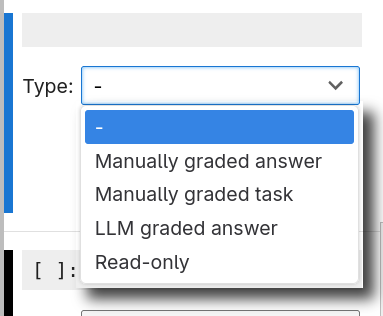
\includegraphics[width=0.8\textwidth]{images/nbgrader_cell.png}
    \caption{Типы ячеек в nbgrader}
    \label{fig:nbgrader-cell}
\end{figure}

\subsection{Создание задания преподавателем}

При подготовке преподавательской версии задания в Jupyter Notebook преподаватель выбирает тип ячейки LLM graded answer и заполняет её с помощью специальных разделителей, принятых в nbgrader:

\begin{itemize}
    \item блок BEGIN QUESTION\_LLM~...~END QUESTION\_LLM содержит формулировку задания, видимую студенту;
    \item блок BEGIN CRITERIA\_LLM~...~END CRITERIA\_LLM содержит эталонный ответ и критерии оценивания, скрытые от студента.
\end{itemize}

Пример разметки ячейки приведён на рис.~\ref{fig:teacher-cell}.

\begin{figure}[h]
    \centering
    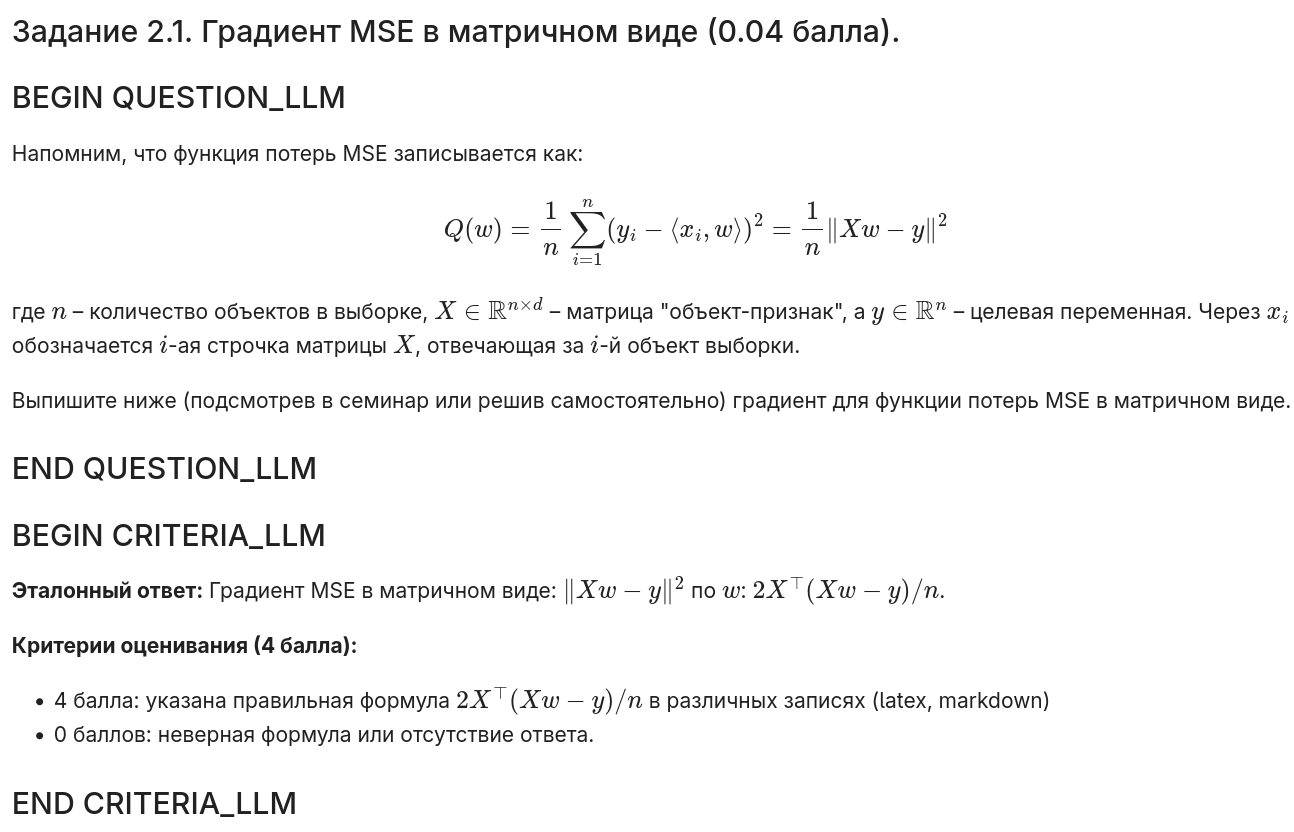
\includegraphics[width=0.8\textwidth]{images/example1.png}
    \caption{Пример ячейки, заполненной преподавателем}
    \label{fig:teacher-cell}
\end{figure}

\subsection{Генерация студенческой версии}

Генерация студенческой версии задания выполняется стандартной командой nbgrader: nbgrader generate\_assignment.

В результате блок с критериями удаляется, а на его месте появляется текст YOUR ANSWER HERE, сохраняя при этом формулировку задания в неизменном виде. Пример отображен на рис.~\ref{fig:student-cell}.

\begin{figure}[h]
    \centering
    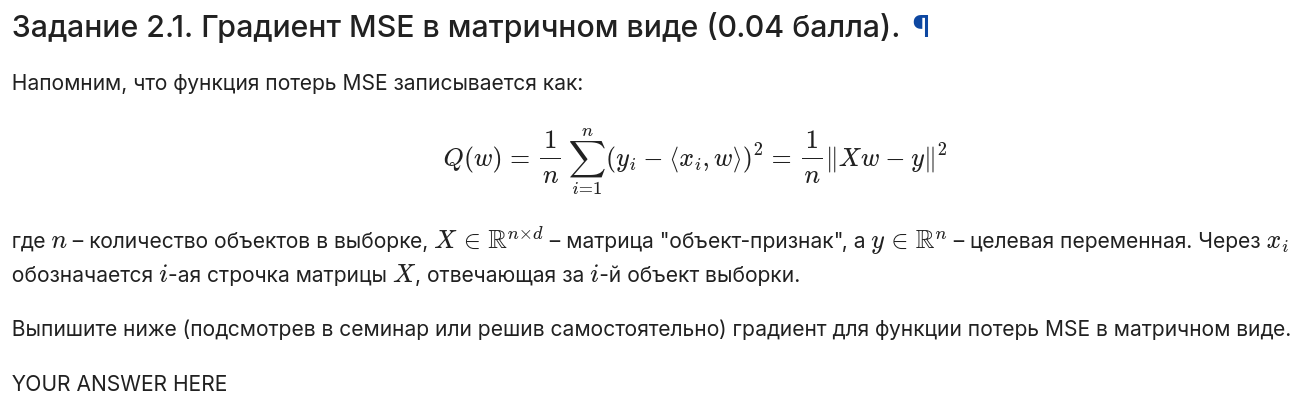
\includegraphics[width=0.8\textwidth]{images/example2.png}
    \caption{Пример ячейки, которую видит студент}
    \label{fig:student-cell}
\end{figure}

\subsection{Конфигурация и запуск проверки}

Перед запуском автоматической проверки преподаватель заполняет конфигурационный файл, задающий параметры обращения к БЯМ. Ключевые поля конфигурации:


\begin{itemize}
    \item llm\_api\_key, llm\_api\_base, llm\_model - параметры подключения к API языковой модели;
    \item БЯМ\_prompt\_template - шаблон промпта, в который подставляются:
        \begin{itemize}
            \item \{question\} - формулировка задания;
            \item \{student\_answer\} - ответ студента;
            \item \{cell\_output\} - вывод ячейки (если есть);
            \item \{grading\_instructions\} - критерии оценивания;
            \item \{max\_points\} - максимальный балл за задание.
        \end{itemize}
    \item begin\_question\_delimiter, end\_question\_delimiter и аналогичные поля для критериев - настройка разделителей разметки; по умолчанию равны BEGIN QUESTION\_LLM и END QUESTION\_LLM для заданий и BEGIN CRITERIA\_LLM и END CRITERIA\_LLM для критериев.
    \item llm\_timeout - максимальное время ожидания ответа от API (в секундах).
\end{itemize}
Модель получает на вход перечисленные данные и возвращает число от 0 до max\_points, представляющее выставленный балл.

После получения ответов студентов преподаватель запускает проверку стандартной командой: nbgrader autograde.

Система автоматически обходит все ячейки типа LLM graded answer, отправляет соответствующие запросы к языковой модели и сохраняет выставленные баллы в базу данных nbgrader. Остальные типы ячеек проверяются штатными механизмами инструмента.

\section{Создание системы для проверки проектов}
